% Figure 1: From contract to execution (WSSE five-page paper)
% 正本＝本file（TikZ・standalone）。単体コンパイル：pdflatex figure1-contract-flow.tex
% 論文へは \input か、コンパイル済みPDFの \includegraphics で取り込む。
% 対応キャプション（草稿en-v1）：Contract → compiler → 6 plans → run time (manifest →
% request assembly → read-only review → verdict transcription → 4 post-checks).
% Sealed records span every stage.
\documentclass[tikz,border=3pt]{standalone}
\usetikzlibrary{arrows.meta,positioning,fit,backgrounds,calc}
\begin{document}
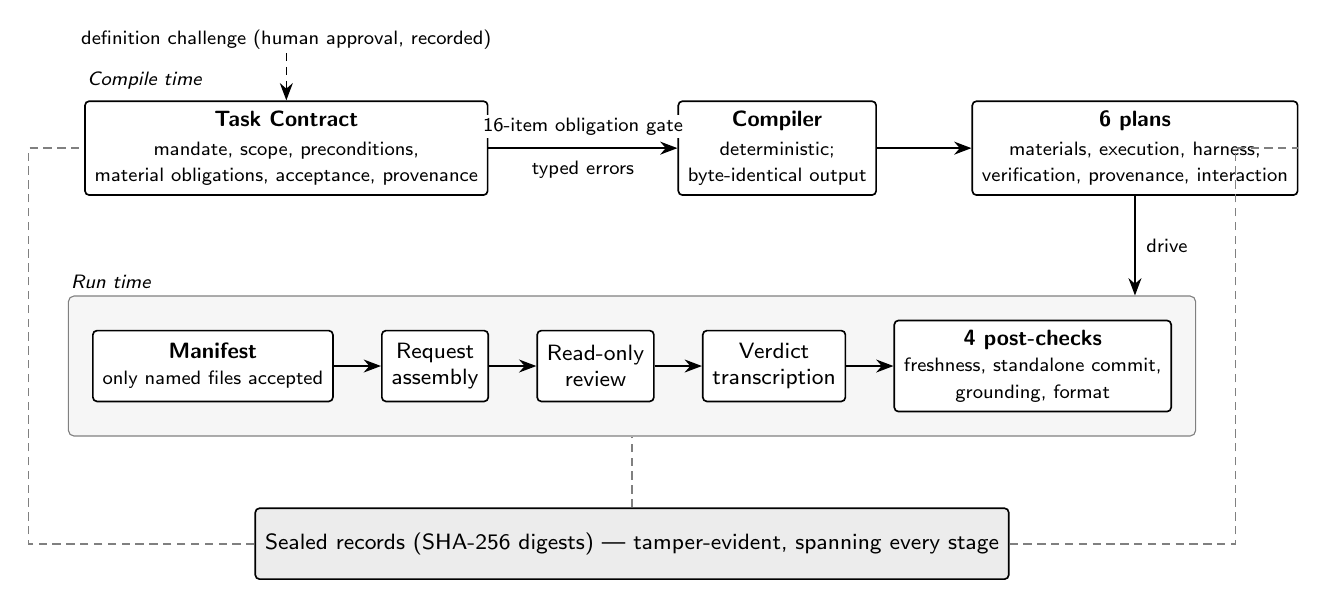
\begin{tikzpicture}[
  font=\footnotesize\sffamily,
  box/.style={draw, semithick, rounded corners=1.5pt, align=center, fill=white,
              inner sep=3.5pt, minimum height=9mm},
  lab/.style={font=\scriptsize\sffamily, align=center, fill=white, inner sep=1pt},
  arr/.style={-{Stealth[length=2.2mm]}, semithick},
  seal/.style={densely dashed, gray, semithick}
]

% ---------- compile time ----------
\node[box] (contract) {\textbf{Task Contract}\\[1pt]
  {\scriptsize mandate, scope, preconditions,}\\
  {\scriptsize material obligations, acceptance, provenance}};
\node[box, right=24mm of contract] (compiler) {\textbf{Compiler}\\[1pt]
  {\scriptsize deterministic;}\\
  {\scriptsize byte-identical output}};
\node[box, right=12mm of compiler] (plans) {\textbf{6 plans}\\[1pt]
  {\scriptsize materials, execution, harness,}\\
  {\scriptsize verification, provenance, interaction}};

\draw[arr] (contract) -- node[lab, above=1.2mm]{16-item obligation gate}
                         node[lab, below=1.2mm]{typed errors} (compiler);
\draw[arr] (compiler) -- (plans);

\node[lab, above=6mm of contract] (defch)
  {definition challenge (human approval, recorded)};
\draw[arr, densely dashed] (defch) -- (contract);

\node[lab, fill=none, anchor=south west] at ($(contract.north west)+(0,1mm)$)
  {\emph{Compile time}};

% ---------- run time ----------
\node[box, below=17mm of contract.south west, anchor=north west, xshift=1mm] (manifest)
  {\textbf{Manifest}\\{\scriptsize only named files accepted}};
\node[box, right=6mm of manifest] (request) {Request\\assembly};
\node[box, right=6mm of request] (review) {Read-only\\review};
\node[box, right=6mm of review] (verdict) {Verdict\\transcription};
\node[box, right=6mm of verdict] (checks) {\textbf{4 post-checks}\\
  {\scriptsize freshness, standalone commit,}\\
  {\scriptsize grounding, format}};

\draw[arr] (manifest) -- (request);
\draw[arr] (request) -- (review);
\draw[arr] (review) -- (verdict);
\draw[arr] (verdict) -- (checks);

\begin{scope}[on background layer]
  \node[draw=gray, rounded corners=2pt, inner sep=3mm, fill=gray!7,
        fit=(manifest)(checks)] (runbox) {};
\end{scope}
\node[lab, anchor=south west, fill=none] at ($(runbox.north west)+(0,0.5mm)$)
  {\emph{Run time}};

\draw[arr] (plans.south) -- node[lab, right=1mm]{drive}
  (plans.south |- runbox.north);

% ---------- sealed records ----------
\node[box, fill=gray!15, below=9mm of runbox] (sealed)
  {Sealed records (SHA-256 digests) --- tamper-evident, spanning every stage};
\coordinate (lx) at ($(runbox.west)+(-5mm,0)$);
\coordinate (rx) at ($(runbox.east)+(5mm,0)$);
\draw[seal] (sealed.north) -- (runbox.south);
\draw[seal] (sealed.west) -| (lx |- contract.west) -- (contract.west);
\draw[seal] (sealed.east) -| (rx |- plans.east) -- (plans.east);

\end{tikzpicture}
\end{document}
